\documentclass{article}
\iffalse
This file is protected by Copyright. Please refer to the COPYRIGHT file
distributed with this source distribution.

This file is part of OpenCPI <http://www.opencpi.org>

OpenCPI is free software: you can redistribute it and/or modify it under the
terms of the GNU Lesser General Public License as published by the Free Software
Foundation, either version 3 of the License, or (at your option) any later
version.

OpenCPI is distributed in the hope that it will be useful, but WITHOUT ANY
WARRANTY; without even the implied warranty of MERCHANTABILITY or FITNESS FOR A
PARTICULAR PURPOSE. See the GNU Lesser General Public License for more details.

You should have received a copy of the GNU Lesser General Public License along
with this program. If not, see <http://www.gnu.org/licenses/>.
\fi

\author{} % Force author to be blank
%----------------------------------------------------------------------------------------
% Paper size, orientation and margins
%----------------------------------------------------------------------------------------
\usepackage{geometry}
\geometry{
	letterpaper,			% paper type
	portrait,				% text direction
	left=.75in,				% left margin
	top=.75in,				% top margin
	right=.75in,			% right margin
	bottom=.75in			% bottom margin
 }
%----------------------------------------------------------------------------------------
% Header/Footer
%----------------------------------------------------------------------------------------
\usepackage{fancyhdr} \pagestyle{fancy} % required for fancy headers
\renewcommand{\headrulewidth}{0.5pt}
\renewcommand{\footrulewidth}{0.5pt}
\rhead{\small{ANGRYVIPER Team}}
%----------------------------------------------------------------------------------------
% Appendix packages
%----------------------------------------------------------------------------------------
\usepackage[toc,page]{appendix}
%----------------------------------------------------------------------------------------
% Defined Commands & Renamed Commands
%----------------------------------------------------------------------------------------
\renewcommand{\contentsname}{Table of Contents}
\renewcommand{\listfigurename}{List of Figures}
\renewcommand{\listtablename}{List of Tables}
\newcommand{\todo}[1]{\textcolor{red}{TODO: #1}\PackageWarning{TODO:}{#1}} % To do notes
\newcommand{\code}[1]{\texttt{#1}} % For inline code snippet or command line
%----------------------------------------------------------------------------------------
% Various packages
%----------------------------------------------------------------------------------------
\usepackage{hyperref} % for linking urls and lists
\usepackage{graphicx} % for including pictures by file
\usepackage{listings} % for coding language styles
\usepackage{rotating} % for sideways table
\usepackage{pifont}   % for sideways table
\usepackage{pdflscape} % for landscape view
%----------------------------------------------------------------------------------------
% Table packages
%----------------------------------------------------------------------------------------
\usepackage{tabularx} % c=center,l=left,r=right,X=fill
\usepackage{float}
\floatstyle{plaintop}
\usepackage[tableposition=top]{caption}
\newcolumntype{P}[1]{>{\centering\arraybackslash}p{#1}}
\newcolumntype{M}[1]{>{\centering\arraybackslash}m{#1}}
%----------------------------------------------------------------------------------------
% Block Diagram / FSM Drawings
%----------------------------------------------------------------------------------------
\usepackage{tikz}
\usetikzlibrary{shapes,arrows,fit,positioning}
\usetikzlibrary{automata} % used for the fsm
%----------------------------------------------------------------------------------------
% Colors Used
%----------------------------------------------------------------------------------------
\usepackage{colortbl}
\definecolor{blue}{rgb}{.7,.8,.9}
\definecolor{ceruleanblue}{rgb}{0.16, 0.32, 0.75}
\definecolor{drkgreen}{rgb}{0,0.6,0}
\definecolor{deepmagenta}{rgb}{0.8, 0.0, 0.8}
\definecolor{cyan}{rgb}{0.0,0.6,0.6}
\definecolor{maroon}{rgb}{0.5,0,0}
%----------------------------------------------------------------------------------------
% Update the docTitle and docVersion per document
%----------------------------------------------------------------------------------------
\def\docTitle{Application Worker Data Sheet}
\def\docVersion{1.0}
%----------------------------------------------------------------------------------------
\date{Version \docVersion} % Force date to be blank and override date with version
\title{\docTitle}
\lhead{\small{\docTitle}}

\def\comp{peak\_detector}
\def\Comp{Peak Detector}
\graphicspath{ {figures/} }

\begin{document}

\section*{Summary - \Comp}
	\begin{tabular}{|c|M{13.5cm}|}
		\hline
		\rowcolor{blue}
		• & • \\
		\hline
		Name & \comp\\
		\hline
		Version & v1.3 \\
		\hline
		Release Date & Feb 2018 \\
		\hline
		Component Library & ocpi.training.components \\
		\hline
		Workers & \comp.rcc, \comp.hdl \\
		\hline
		Tested Platforms & c7-x86\_64, linux-x13\_3-arm, xsim, isim, Matchstiq-Z1(PL)(Vivado 2017.1 and ISE 14.7) \\
		\hline
	\end{tabular}
\section*{Functionality}
\begin{flushleft}
The {\Comp} worker utilizes the OCPI \textit{iqstream\_protocol} for both input and output ports. The \textit{iqstream\_protocol} defines an interface of 16-bit complex signed samples. The worker calculates the maximum and minimum peaks of the I/Q data arriving at its input port, and passes the input data through to the output port.
\newline

The {\Comp} worker uses two local variables to keep track of the maximum and minimum peak amplitudes. To ensure the peaks are detected correctly, the variable used to keep track of the maximum peak is initialized to the most negative value represented in a signed 16-bit number (-32768), and the minimum peak is initialized to the most positive value represented in a signed 16-bit number (32767). \newline

Upon completion, the {\Comp} returns the most positive I or Q sample value with the \verb+max_peak+ property and the most negative with the \verb+min_peak+ property. \textit{This is not the value of the vector represented by I and Q, but simply the max/min value of the I and Q samples taken independently.}\newline

\end{flushleft}

\section*{Block Diagrams}
	\subsection*{Top level}
\begin{center}
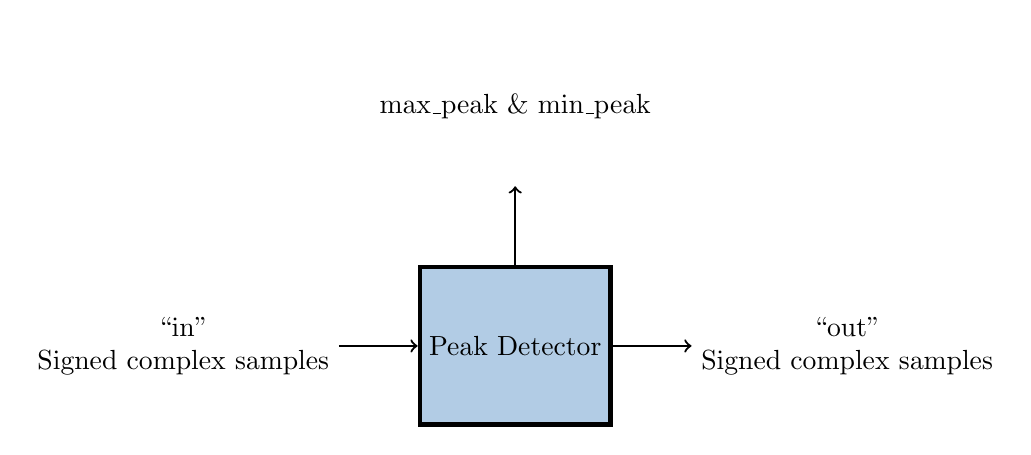
\begin{tikzpicture}[% List of styles applied to all, to override specify on a case-by-case
					every node/.style={
						align=center,  		% use this so that the "\\" for line break works
						minimum size=2cm	% creates space above and below text in rectangle
						},
					every edge/.style={draw,thick}
					]
\node[rectangle,ultra thick,draw=black,fill=blue](R2){\Comp};
\node[rectangle,draw=white,fill=white](R3)[left= of R2]{``in" \\ Signed complex samples};
\node[rectangle,draw=white,fill=white](R4)[right= of R2]{``out" \\ Signed complex samples};
\node[rectangle,draw=white,fill=white](R5)[above= of R2]{max\_peak \& min\_peak};
\path[->]
(R3)edge []	node [] {} (R2)
(R2)edge []	node [] {} (R4)
(R2)edge []	node [] {} (R5)
;
\end{tikzpicture}
\end{center}
\subsection*{State Machine}
\begin{flushleft}
	No finite-state machines (FSM) are implemented by this worker.
\end{flushleft}

\section*{Source Dependencies}
\subsection*{\comp.rcc}
	\begin{itemize}
		\item training\_project/components/\comp.rcc/\comp.cc
	\end{itemize}
\subsection*{\comp.hdl}
	\begin{itemize}
		\item training\_project/components/\comp.hdl/\comp.vhd
	\end{itemize}

\begin{landscape}
\section*{Component Spec Properties}

\begin{flushleft}

	\begin{scriptsize}
	\begin{tabular}{|p{1.5cm}|p{1.5cm}|p{1.5cm}|p{1.5cm}|p{2cm}|p{1cm}|p{1.5cm}|p{2cm}|p{1.5cm}|p{5cm}|}
		\hline
		\rowcolor{blue}
		Name & OCS & OWD RCC & OWD HDL & Type & Length  & Accessibility & Valid Range & Default & Usage \\
		\hline
		\verb+max_peak+ & Property & N/A & N/A & short scalar & N/A & Volatile & -32768 to 32767 & N/A & Used to return the maximum amplitude value\\
		\hline
		\verb+min_peak+ & Property & N/A & N/A & short scalar & N/A & Volatile & -32768 to 32767 & N/A & Used to return the minimum amplitude value\\
		\hline
	\end{tabular}
	\end{scriptsize}


\end{flushleft}

\section*{Worker Properties}
		N/A

\section*{Component Ports}

		\scriptsize
		\begin{tabular}{|M{2cm}|M{1cm}|M{4cm}|c|M{13.5cm}|}
			\hline
			\rowcolor{blue}
			Name & Producer & Protocol & Optional & Usage\\
			\hline
			in
			& false
			& \verb+iqstream_protocol+
			& false
			& I(31:16); Q(15:0); DataWidth=32; If (DATA\_WIDTH\_p $<$ 16), then the data must be signed extended \\
			\hline
			out
			& true
			& \verb+iqstream_protocol+
			& false
			& I(31:16); Q(15:0); DataWidth=32; If (DATA\_WIDTH\_p $<$ 16), then the data must be signed extended \\
			\hline
		\end{tabular}

\section*{Worker Interfaces}
\subsection*{\comp.hdl}
\begin{scriptsize}
\begin{tabular}{|M{2cm}|M{1.5cm}|c|c|M{12cm}|}
             \hline
             \rowcolor{blue}
             Type            & Name & DataWidth & Advanced                & Usage                  \\
             \hline
             StreamInterface & in   & 32        & N/A & Signed complex samples \\
            \hline
            StreamInterface & out  & 32        & N/A & Signed complex samples \\
            \hline
\end{tabular}
\end{scriptsize}
\end{landscape}

\section*{Control Timing and Signals}
\begin{flushleft}
The {\Comp} worker uses the clock from the Control Plane and standard Control Plane signals.
\end{flushleft}

\section*{Performance and Resource Utilization}
	\subsubsection*{\comp.hdl}
    Table entries are a result of building the worker with default parameters:\
        \newline\newline
        \scriptsize
        \begin{tabular}{|c|c|c|c|c|c|c|c|}
                \hline
                \rowcolor{blue}
                Device & Registers & LUTs & Fmax & Memory/Special Functions & Design Suite \\
                \hline
                Zynq XC7Z010-3-CLG400 & 159 & 249 & 516.627 MHz & N/A  & ISE 14.7 \\
                \hline
                Zynq XC7Z020-1-CLG484    & 162    & 153 & 345.781 MHz & N/A & Vivado 2017.1 \\
                \hline
        \end{tabular}

\section*{Test and Verification}
\normalsize

\begin{flushleft}

A single test case is implemented to validate the {\comp} component. An input file is generated (via \textit{generate.py}) containing complex signed 16-bit samples with a tone at 13 Hz. The input data is passed through the worker, so the output file should be identical to the input file. The worker measures the minimum and maximum amplitudes found within the complex data stream. These values, reported as properties, are compared with min/max calculations performed during verification (\textit{verify.py}).


        \begin{figure}[ht]
        \centering
                \begin{minipage}{.5\textwidth}
                        \centering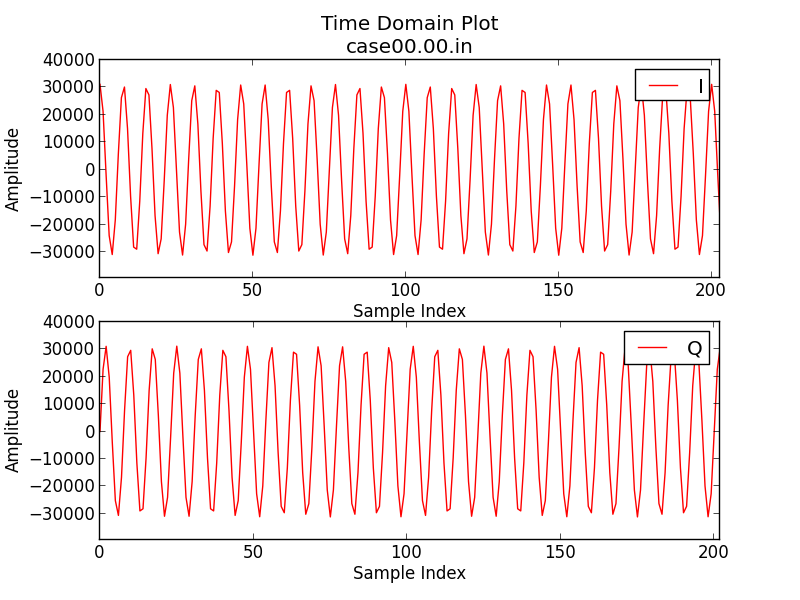
\includegraphics[width=1.0\linewidth]{input_time}
                        \captionof{figure}{Input Time Domain Tone}
                        \label{fig:in_time_tone}
                \end{minipage}%
                \begin{minipage}{.5\textwidth}
                        \centering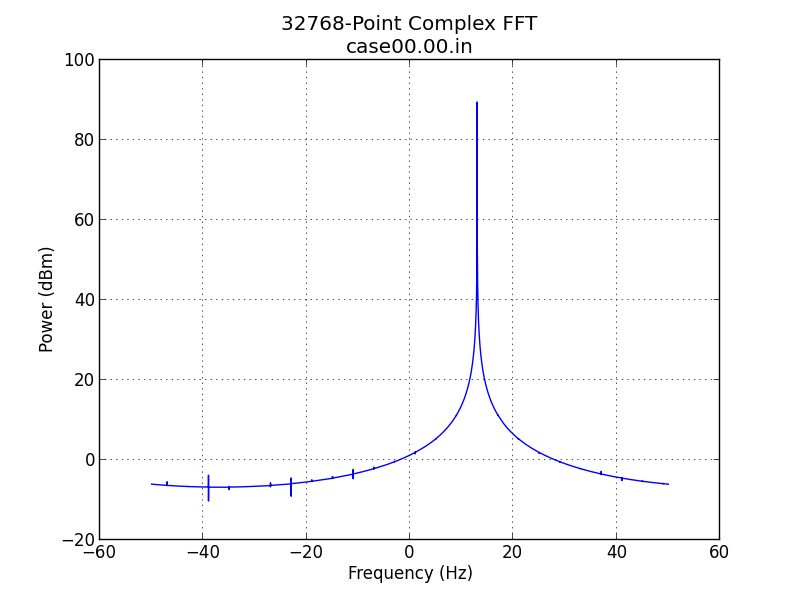
\includegraphics[width=1.0\linewidth]{input_freq}
                        \captionof{figure}{Input Frequency Domain Tone}
                        \label{fig:in_freq_tone}
                \end{minipage}
        \end{figure}


\begin{flushleft}
The output file is first checked that the data is not all zero, and is then checked for the expected length of 32,768 complex samples. Once these quick checks are made the minimum and maximum values are calculated from the file and then compared with the UUT reported values. Figures \ref{fig:out_time_tone} and \ref{fig:out_freq_tone} depict the output of the {\Comp} worker, where the time domain plot displays the first 200 complex samples.
\end{flushleft}
\newpage

        \begin{figure}[ht]
        \centering
                \begin{minipage}{.5\textwidth}
                        \centering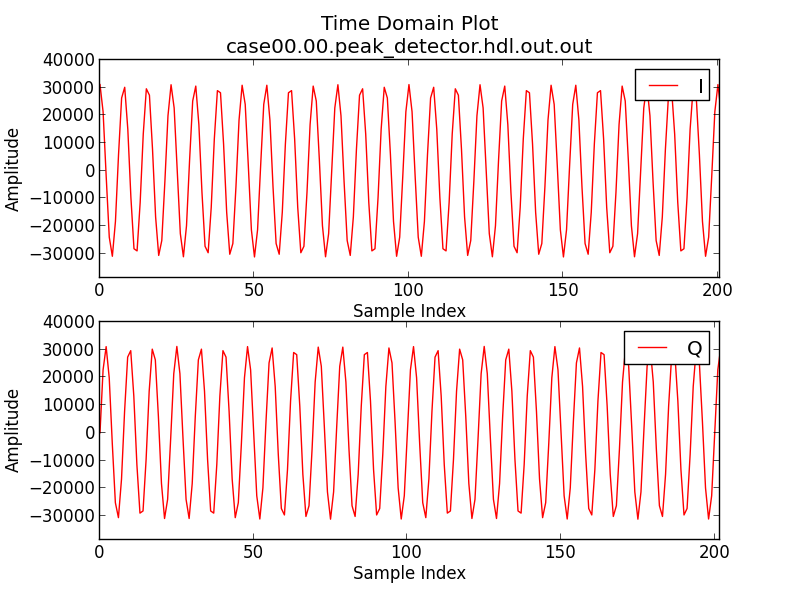
\includegraphics[width=1.0\linewidth]{output_time}
                        \captionof{figure}{Output Time Domain Tone}
                        \label{fig:out_time_tone}
                \end{minipage}%
                \begin{minipage}{.5\textwidth}
                        \centering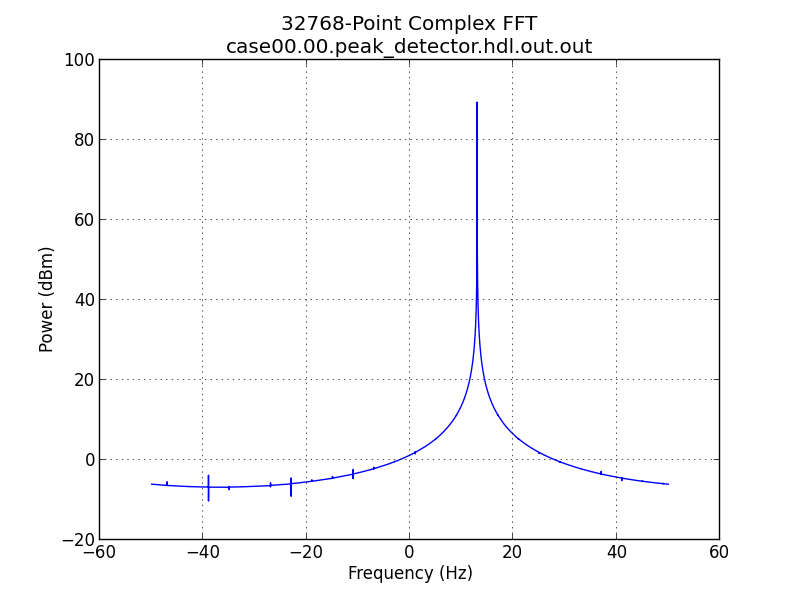
\includegraphics[width=1.0\linewidth]{output_freq}
                        \captionof{figure}{Output Frequency Domain Tone}
                        \label{fig:out_freq_tone}
                \end{minipage}
        \end{figure}
\end{flushleft}
\end{document}
